% !TEX program = pdflatex
\documentclass[3p,11pt]{elsarticle}
\usepackage{amsmath,amssymb}
\usepackage{array}
\usepackage{booktabs}
\usepackage[tableposition=top]{caption}
\usepackage{graphicx}
\usepackage{url}
\urlstyle{same}
\usepackage[hidelinks]{hyperref}
\emergencystretch=3em
% first-page footer: the page number alone
\makeatletter
\def\ps@pprintTitle{\let\@oddhead\@empty\let\@evenhead\@empty
  \def\@oddfoot{\hfil\thepage\hfil}\let\@evenfoot\@oddfoot}
\makeatother

% ---- notation ---------------------------------------------------------------
\newcommand{\kms}{km\,s$^{-1}$}
\newcommand{\ms}{m\,s$^{-1}$}
\newcommand{\Msun}{M$_\odot$}
\newcommand{\Rsun}{R$_\odot$}
\newcommand{\Mearth}{M$_\oplus$}

\begin{document}

\begin{frontmatter}

\title{A compact system of four sub-Neptune-mass planets around HD\,32564 in public HARPS velocities}

\author{Charles C. Norton}

\begin{abstract}
HD\,32564 (HIP\,23575) is a G6 dwarf of 0.92\,\Msun\ at 48.5\,pc, old and magnetically quiet. HARPS
observed it on 193 nights between 2009 and 2016, and its public velocities carry four Keplerian
signals, at 2.5566, 11.063, 23.61 and 49.13\,d, with semi-amplitudes of 4.2, 3.5, 3.0 and
1.7\,\ms: four planets with minimum masses of 8.5, 11.4, 12.5 and 9.4\,\Mearth\ within 0.26\,au of
the star. Each signal stands in three reductions of the same spectra, SERVAL's velocities, the HARPS
pipeline's cross-correlation velocities and line-by-line velocities measured here, the last from all
lines and from the lines whose shifts do not follow the Ca\,{\sc ii} H and K index alike, and each keeps
its amplitude and phase from the first half of the nights to the second. None of eight activity
indicators has power at any of the four periods. A refit and simulations of the observing window
reject the innermost signal's daily alias, whose peak lies at 1.635\,d, and every planet's one-year
aliases; N-body integrations keep the system stable for $10^6$ orbits of the innermost planet on
circular orbits, and TESS sees no transits. A fifth signal, at 123.0\,d and 1.1\,\ms, improves the fit
by $\Delta\mathrm{BIC} = 26$ in SERVAL's velocities and stands in the pipeline's at a false-alarm level
of 0.05; it is a candidate, and the five-planet system stays quasi-periodic only if its orbits are close
to circular.
\end{abstract}

\begin{keyword}
Techniques: radial velocities \sep Planets and satellites: detection \sep Planetary systems \sep
Stars: individual: HD\,32564
\end{keyword}

\end{frontmatter}

\section{Introduction}\label{sec:intro}

Compact systems of planets between the Earth's and Neptune's mass, several of them within a few tenths
of an astronomical unit of a Sun-like star, are among the commonest planetary systems in the Galaxy. The
transit surveys found them in hundreds, their planets alike in size and evenly spaced~\cite{Weiss2018},
their neighbouring periods often a little wide of the low-order resonances~\cite{Fabrycky2014}; the
radial-velocity surveys weigh the nearby ones. HARPS has watched several thousand nearby stars since
2003, and HARPS-RVBank~\cite{Trifonov2020} recomputed every public HARPS velocity with
SERVAL~\cite{Zechmeister2018}, corrected the instrument's nightly zero points and attached each
spectrum's activity indicators, so that each star's whole record can be read at once.

HD\,32564 is one of those stars. Its velocities were taken on 193 nights between 2009 and 2016, and no
planet has been reported around it. Section~\ref{sec:data} describes the data,
Section~\ref{sec:star} the star, Section~\ref{sec:signals} the signals and the models that hold them,
Section~\ref{sec:tests} the tests against stellar activity and the instrument,
Section~\ref{sec:orbits} the orbits, masses and dynamics, and Section~\ref{sec:discussion} the
system's architecture.

\section{Data}\label{sec:data}

HARPS-RVBank holds 205 velocities of HD\,32564 from 193 nights between 2009 November 29 and 2016
March 18, with a median error of 1.05\,\ms; seven nights follow HARPS's fibre upgrade of 2015 June,
across which the velocities take an offset of their own. The velocities of each night are averaged,
weighted by their inverse variances. The same spectra give two further sets of velocities. DACE holds
the HARPS pipeline's cross-correlation velocities, 195 nights after the pipeline's quality control,
with the Mount Wilson S index of each spectrum. The third set was measured here from the ESO Science
Archive's HARPS spectra, the one of highest signal to noise from each of 199 nights: every spectrum is
put on a grid uniform in log wavelength at 0.4\,\kms\ from 3800 to 6880\,\AA\ in the star's frame,
the median spectrum is the template, and each spectrum's shift in each of the template's 4\,022 lines
deeper than 4 per cent is Bouchy's derivative estimate~\cite{Bouchy2001} with its photon error. A
spectrum's velocity is the weighted mean of its lines, lines more than $5\sigma$ from the median set
aside and each line carrying a jitter of its own, in the manner of line-by-line
velocimetry~\cite{Artigau2022}. Each line's shifts are correlated with the S index measured in the same
spectra, and the 303 lines whose correlation passes $p < 0.01$ are left out of a second velocity, made
from the 3\,719 quiet lines. The activity indicators are the bank's chromatic index, differential line width,
H$\alpha$ and Na\,D indices and the pipeline's line width and bisector, and the S index from DACE and
from the line-by-line spectra. The star's TESS light
curves~\cite{Ricker2015}, sectors 5, 32 and 98 at two-minute or 20-second cadence from SPOC, come
through Lightkurve~\cite{Lightkurve2018}.

\section{The star}\label{sec:star}

Table~\ref{tab:star} gives the star's parameters. Gaia DR3~\cite{GaiaDR3} places it at
$48.47 \pm 0.04$\,pc with a renormalised unit weight error of 0.97 and no non-single-star solution,
and its astrophysical parameters~\cite{Creevey2023} give a G dwarf of 5\,550\,K, solar metallicity,
0.92\,\Msun\ and 0.96\,\Rsun, 8.6\,Gyr old. The S index of its 207 HARPS spectra is $0.169 \pm 0.004$,
$\log R'_\mathrm{HK} = -4.96$ for $B-V = 0.70$~\cite{Noyes1984}, the activity of an old, slowly
rotating star; the activity-rotation relation~\cite{Mamajek2008} gives a rotation period near 31\,d. In
TESS's sectors 5 and 32 its light varies by less than 30\,ppm, sector 98 carries the 13-day pattern of
the spacecraft's orbit, and no rotation shows in any of them.

\begin{table}[!htbp]
\centering
\caption{HD\,32564.}\label{tab:star}
\begin{tabular}{l r l}
\toprule
Parameter & Value & Source \\
\midrule
Gaia DR3 & 3227308623164447616 & \cite{GaiaDR3} \\
$G$, $G_\mathrm{BP} - G_\mathrm{RP}$ (mag) & 8.42, 0.89 & \cite{GaiaDR3} \\
Parallax (mas) & $20.631 \pm 0.017$ & \cite{GaiaDR3} \\
RUWE & 0.97 & \cite{GaiaDR3} \\
$T_\mathrm{eff}$ (K) & 5\,550 & \cite{Creevey2023} \\
$\log g$ & 4.40 & \cite{Creevey2023} \\
$[\mathrm{M/H}]$ & $-0.06$ & \cite{Creevey2023} \\
Mass (\Msun) & $0.92 \pm 0.04$ & \cite{Creevey2023} \\
Radius (\Rsun) & $0.957 \pm 0.020$ & \cite{Creevey2023} \\
Age (Gyr) & $8.6^{+1.4}_{-2.0}$ & \cite{Creevey2023} \\
S index & $0.169 \pm 0.004$ & HARPS, DACE \\
$\log R'_\mathrm{HK}$ & $-4.96$ & this work \\
\bottomrule
\end{tabular}
\end{table}

\section{The signals}\label{sec:signals}

\subsection{Periodograms}

A generalised Lomb-Scargle periodogram~\cite{Zechmeister2009} of SERVAL's velocities from 1.2 to
3\,000\,d, with the offset across the fibre upgrade fitted, peaks at 2.557\,d at a false-alarm
level~\cite{Baluev2008} of $10^{-15}$. With that signal's sinusoid fitted, the residuals peak at
11.062\,d ($4 \times 10^{-18}$), then at 23.596\,d ($10^{-22}$), at 49.149\,d ($7 \times 10^{-13}$)
and at 123.0\,d ($10^{-5}$); with all five fitted, the highest peak, at 1.393\,d, stands at a
false-alarm level of 0.2 (Figure~\ref{fig:periodograms}).

\begin{figure}[!htbp]
\centering
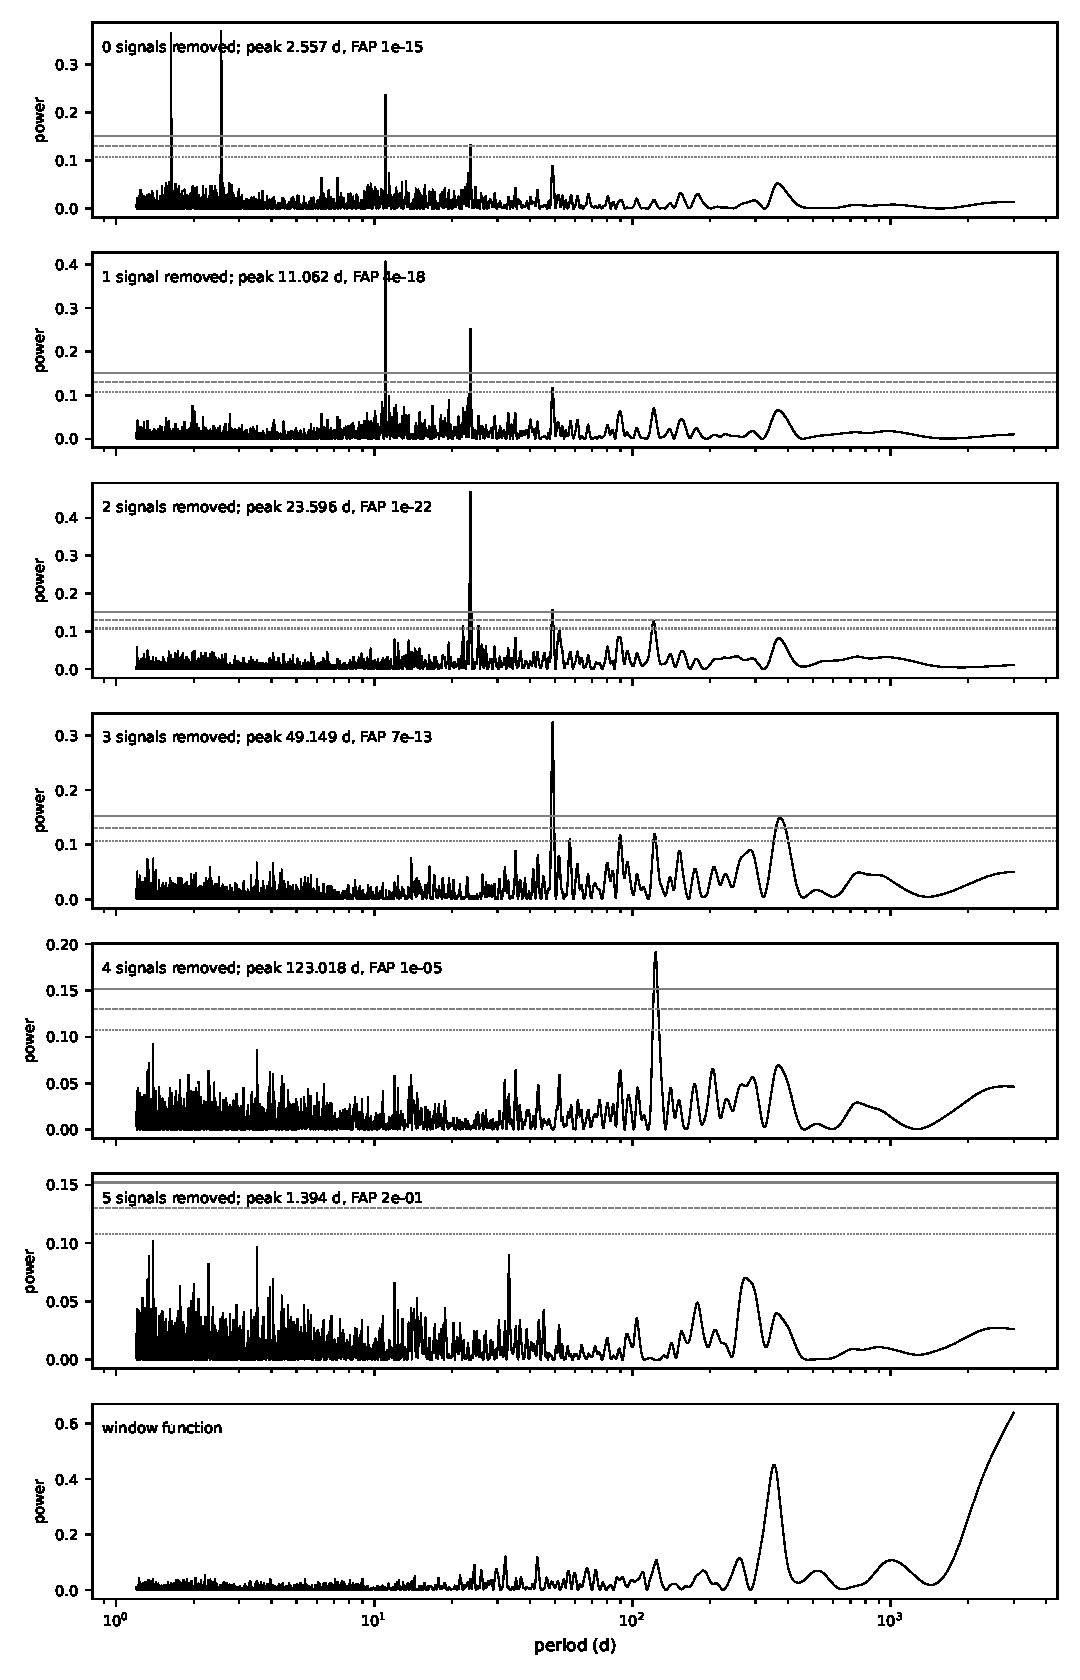
\includegraphics[width=0.92\textwidth]{periodograms.pdf}
\caption{Generalised Lomb-Scargle periodograms of SERVAL's nightly velocities of HD\,32564, each with
the sinusoids of the signals above it fitted jointly. The horizontal lines are the false-alarm levels of
0.1, 0.01 and 0.001.}\label{fig:periodograms}
\end{figure}

\subsection{Models}

Keplerian models of three to six planets were fitted by least squares from the periodograms' periods,
each with an offset on each side of the fibre upgrade and a jitter added to the errors
(Table~\ref{tab:models}). With every orbit circular, the fourth planet lowers the Bayesian information
criterion~\cite{Schwarz1978} by 64 and the fifth by a further 26; a sixth, at 1.393\,d, lowers it by 4,
which does not support it. Free eccentricities improve the log-likelihood of the four-planet model by
less than 0.1 and of the five-planet model by 2.0 for ten parameters, so the circular models are
preferred.

\begin{table}[!htbp]
\centering
\caption{Keplerian models of SERVAL's velocities of HD\,32564: log-likelihood with free and with
circular orbits, the Bayesian information criterion of each, the free model's jitter and its residual
scatter.}
\label{tab:models}
\small
\begin{tabular}{c r r r r r r}
\toprule
Planets & $\ln L$ & $\ln L$ (circular) & BIC & BIC (circular) & Jitter (\ms) & Scatter (\ms) \\
\midrule
3 & $-418.1$ & $-420.1$ & 930.9 & 903.4 & 1.84 & 2.11 \\
4 & $-380.2$ & $-380.2$ & 881.5 & 839.3 & 1.41 & 1.75 \\
5 & $-357.1$ & $-359.1$ & 861.5 & 812.9 & 1.15 & 1.55 \\
6 & $-339.8$ & $-349.0$ & 853.3 & 808.6 & 0.97 & 1.43 \\
\bottomrule
\end{tabular}
\end{table}

\subsection{The innermost period}

The 2.5566-d signal's daily alias, at $|1/P - 1/\mathrm{d}|$, has its peak in SERVAL's velocities at
1.635\,d, two cycles a year from the exact alias at 1.650\,d, where the window's yearly sidelobes move
it; with the other three signals fitted it carries 0.90 of the period's power, 0.681 against 0.759.
Refitted with the innermost planet at 1.635\,d, the four-planet model loses 31.2 in log-likelihood. The
observing window decides as well~\cite{Dawson2010}. Three hundred sets of velocities drawn at the
observed times from the four-planet model with the fitted jitter, with the innermost planet at
2.5566\,d, give a ratio of the two peaks' powers of $1.17 \pm 0.04$, and 72 per cent of them reach the
observed 1.14; three hundred with the planet at 1.635\,d give $0.87 \pm 0.03$, and none reaches it.
The period is 2.5566\,d. The one-year aliases of the other three planets, at 10.72 and 11.42, 22.12 and
25.30, and 43.05 and 57.26\,d, fit worse by 91, 88, 73, 67, 31 and 29 in log-likelihood.

\subsection{The fifth signal}

The 123-d signal stands at a false-alarm level of $10^{-5}$ in SERVAL's velocities with the four
planets fitted, and in the pipeline's velocities its peak, at 124.0\,d, stands at 0.05. It is a
candidate. Fitted with free eccentricities, it takes 0.19 and the 49-d planet 0.20, and the
five-planet system then turns chaotic (Section~\ref{sec:orbits}).

\section{Activity and the instrument}\label{sec:tests}

\subsection{Three reductions}

Table~\ref{tab:reductions} gives each signal in each of the three reductions, found in the residuals of
the other three signals, with its semi-amplitude fitted to the first and to the second half of the nights
apart. SERVAL fits a template to every spectrum's whole extracted orders, the pipeline cross-correlates a
binary mask, and the line-by-line velocities weigh each line by its own scatter, so a signal one
reduction made would not stand in the others; all four stand in all three, with the same phase in the two
halves of each and amplitudes that agree within twice their errors. They stand at the same strength in
the velocities of the 3\,719 lines whose shifts do not follow the S index as in those of all 4\,022, as
they would not if the activity-sensitive lines carried them.

\begin{table}[!htbp]
\centering
\caption{The four signals of HD\,32564 in three reductions of its HARPS spectra: each signal's
false-alarm level in the residuals of the other three, and its semi-amplitude (\ms) in the first and
second half of the nights.}\label{tab:reductions}
\small
\begin{tabular}{l c c c c}
\toprule
Reduction & 2.5566\,d & 11.063\,d & 23.61\,d & 49.2\,d \\
\midrule
SERVAL (193 nights) & $2\times10^{-60}$ & $10^{-45}$ & $2\times10^{-33}$ & $4\times10^{-17}$ \\
& 4.0, 4.6 & 3.4, 3.4 & 2.7, 2.8 & 1.7, 1.7 \\
Pipeline (195 nights) & $10^{-59}$ & $2\times10^{-41}$ & $6\times10^{-33}$ & $4\times10^{-7}$ \\
& 4.1, 4.5 & 3.5, 3.2 & 2.7, 2.9 & 1.2, 1.3 \\
Line-by-line, all lines (199) & $4\times10^{-28}$ & $7\times10^{-16}$ & $10^{-14}$ & $10^{-5}$ \\
& 4.1, 4.4 & 3.1, 3.3 & 3.1, 3.4 & 1.7, 2.3 \\
Line-by-line, quiet lines (199) & $10^{-26}$ & $9\times10^{-15}$ & $10^{-13}$ & $2\times10^{-5}$ \\
& 4.1, 4.2 & 3.0, 3.3 & 3.0, 3.4 & 1.7, 2.4 \\
\bottomrule
\end{tabular}
\end{table}

\subsection{Activity indicators}

The periodograms of the chromatic index, the differential line width, the H$\alpha$ and Na\,D indices,
the pipeline's line width and bisector, the S index from DACE's spectra and from the line-by-line spectra
have no power at any of the four periods: within 5 per cent of each, no indicator's highest peak stands
below a false-alarm level of 0.99. Their own highest peaks lie at a year (H$\alpha$ and Na\,D), at four
years (the chromatic index) and at the longest periods searched (the line width and bisector), and
neither S index has a significant peak at all. The star's rotation, near 31\,d, matches none of the
periods or their harmonics.

\subsection{TESS}

Box least squares within 2 per cent of each period finds no transit in the three sectors: at 2.5566\,d
the best box's 39 events, measured one by one, have a median depth of 35\,ppm, where a planet of
9\,\Mearth\ and 2.5 to 3 Earth radii would take 600 to 800\,ppm from every one. The four planets' transit
probabilities are 13, 5, 3 and 2 per cent.

\section{Orbits, masses and stability}\label{sec:orbits}

Table~\ref{tab:orbits} gives the planets' orbits, sampled with emcee~\cite{ForemanMackey2013} and its
differential-evolution moves~\cite{terBraak2006} from SERVAL's nightly velocities, each orbit circular,
with an offset on each side of the fibre upgrade, a jitter added to the errors and the star's mass of
0.917\,\Msun. Sampled with the fifth signal in the model, the four planets keep their values within
their errors, and the fifth has a period of $122.96 \pm 0.69$\,d, a semi-amplitude of
$1.13 \pm 0.17$\,\ms\ and a minimum mass of $8.3 \pm 1.2$\,\Mearth\ at 0.47\,au.
Figure~\ref{fig:phased} shows each planet's orbit with the others' removed.

\begin{table}[!htbp]
\centering
\caption{The planets of HD\,32564: medians and 68 per cent intervals of the circular orbits sampled from
SERVAL's velocities, with the star's mass of 0.917\,\Msun. The jitter is $1.46 \pm 0.10$\,\ms.}
\label{tab:orbits}
\begin{tabular}{l r r r r}
\toprule
Planet & Period (d) & $K$ (\ms) & $m \sin i$ (\Mearth) & $a$ (au) \\
\midrule
HD\,32564\,b & $2.55660 \pm 0.00010$ & $4.22 \pm 0.16$ & $8.5 \pm 0.3$ & 0.0356 \\
HD\,32564\,c & $11.0634 \pm 0.0018$ & $3.46 \pm 0.16$ & $11.4 \pm 0.5$ & 0.0944 \\
HD\,32564\,d & $23.613 \pm 0.011$ & $2.95 \pm 0.16$ & $12.5 \pm 0.7$ & 0.157 \\
HD\,32564\,e & $49.13 \pm 0.07$ & $1.74 \pm 0.16$ & $9.4 \pm 0.9$ & 0.255 \\
\bottomrule
\end{tabular}
\end{table}

Integrated with REBOUND~\cite{Rein2012} and its WHFast integrator~\cite{Rein2015} for $10^6$ orbits of
the innermost planet, some 7\,000\,yr, coplanar and edge-on at the minimum masses, the four- and
five-planet systems on circular orbits stay bounded with a MEGNO~\cite{Cincotta2000} of 2.0, the value
of quasi-periodic motion. The four-planet fit with free eccentricities settles on circular orbits. The
five-planet fit with them gives the 49-d planet and the fifth signal eccentricities of 0.20 and 0.19,
and that system, though bounded over the integration, turns chaotic, its MEGNO reaching 4.5. Adjacent
planets on circular orbits are separated by 32, 17 and 17 of their mutual Hill radii, and the fifth
signal's orbit by 22 from the fourth.

The four-planet residuals bound what else the velocities hold (Figure~\ref{fig:limits}). A circular
orbit is recovered 90 per cent of the time at a semi-amplitude of 1.1 to 1.9\,\ms\ out to 200\,d, a
minimum mass of 2.4 to 3.0\,\Mearth\ at 1.5 to 2.7\,d, 3.4 to 4.1\,\Mearth\ at 3 to 9\,d, 4.6 to
7\,\Mearth\ at 10 to 34\,d, 7.3 to 8.9\,\Mearth\ at 41 to 74\,d and 10 to 14\,\Mearth\ at 90 to
200\,d. From 240 to 520\,d the limit lies at 22 to 33\,\Mearth, near 430\,d at 99\,\Mearth, and beyond
600\,d no semi-amplitude up to 15\,\ms\ is recovered 90 per cent of the time.

\begin{figure}[!htbp]
\centering
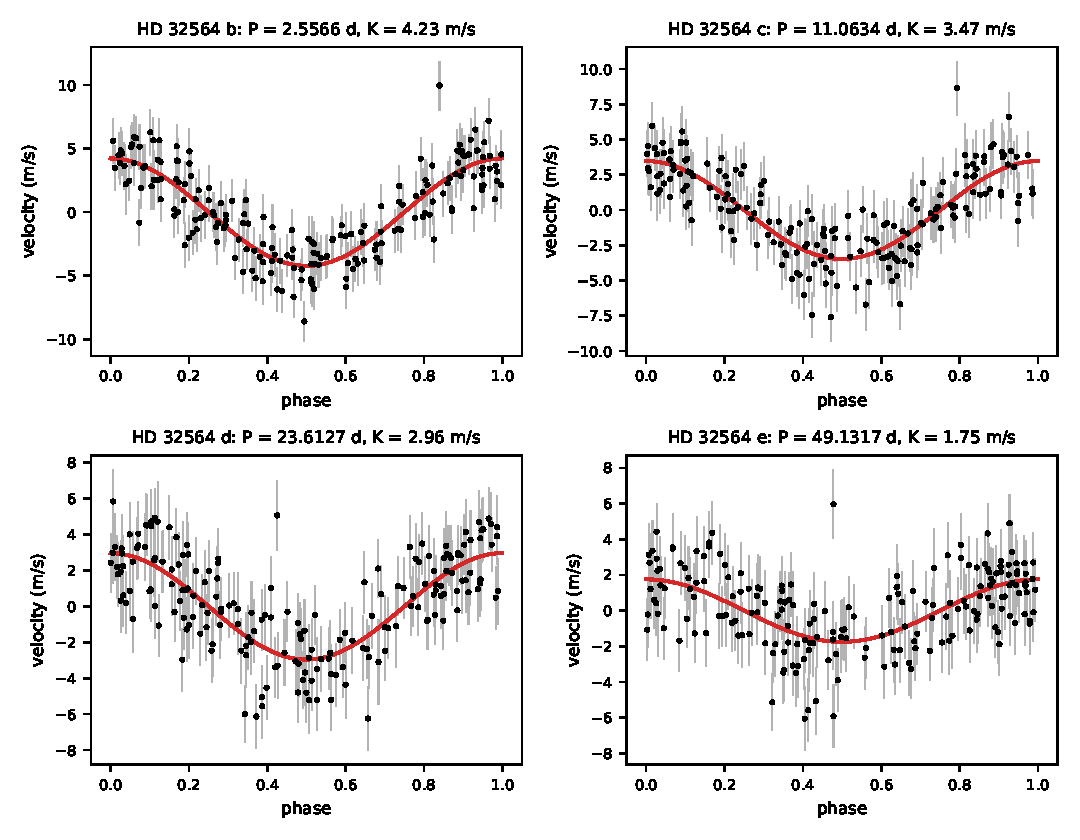
\includegraphics[width=0.92\textwidth]{phased.pdf}
\caption{SERVAL's nightly velocities of HD\,32564 phased at each planet's period, the other planets'
orbits removed, with the circular orbit.}\label{fig:phased}
\end{figure}

\begin{figure}[!htbp]
\centering
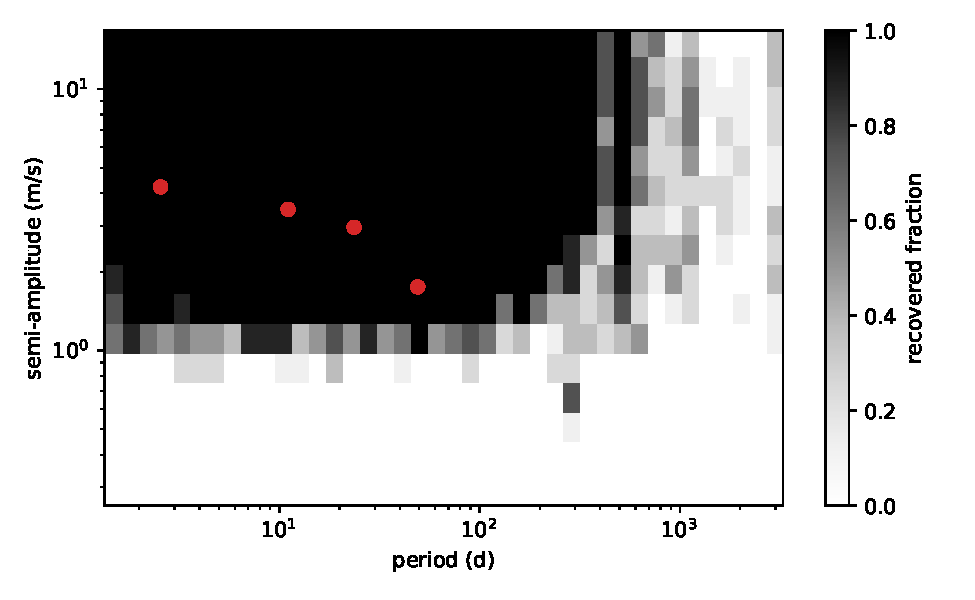
\includegraphics[width=0.8\textwidth]{detection_limits.pdf}
\caption{The fraction of circular orbits injected into the four-planet residuals that are recovered,
the highest peak of the residual periodogram within 2 per cent of the injected period at a false-alarm
level below $10^{-3}$, eight phases at each period and semi-amplitude. The four planets are
marked.}\label{fig:limits}
\end{figure}

\section{Discussion}\label{sec:discussion}

HD\,32564's four planets are alike: their minimum masses lie between 8.5 and 12.5\,\Mearth, and
they sit at 0.036, 0.094, 0.157 and 0.255\,au from a star of 0.78 solar luminosities, where they receive
620, 88, 32 and 12 times the Earth's insolation. The outer three are spaced nearly evenly in the
logarithm of their periods, at ratios of 2.13 and 2.08, each a few per cent wide of the 2:1 resonance,
as neighbouring planets in the transiting multi-planet systems most often are~\cite{Fabrycky2014}; the
alikeness of masses and spacing is the pattern those systems show in their sizes~\cite{Weiss2018}. The
ratio between the innermost two, 4.33, is the system's widest: a planet midway, near 5.3\,d, would
continue the spacing of the outer three, and the velocities hold none above 3.8\,\Mearth\ there. The
fifth signal, at 123.0\,d, would extend the sequence at a ratio of 2.50.

With minimum masses of 8.5 to 12.5\,\Mearth, the planets are heavier than the Earth-like rocky planets and
lie where sub-Neptunes with gaseous envelopes are common. None transits for TESS; the innermost
planet's transit probability is 13 per cent, and in a coplanar system the outer planets, at 5, 3 and 2
per cent, could transit only where it does.

\section{Conclusion}\label{sec:conclusion}

HD\,32564, a quiet G6 dwarf at 48.5\,pc, hosts four planets of 8.5 to 12.5\,\Mearth\ on orbits
of 2.5566, 11.063, 23.61 and 49.1\,d, read from 193 nights of public HARPS velocities. Each planet
stands in three reductions of the same spectra and in the activity-quiet lines alone, keeps its
amplitude and phase across the data, and has no counterpart in eight activity indicators; the
innermost period is the true one against its daily alias, and the system is stable on circular orbits.
A fifth signal at 123.0\,d is a candidate. Velocities from another instrument would test it, and would
measure the four planets' eccentricities, which the dynamics already hold close to zero.

\section*{Acknowledgements}

Based on data obtained from the ESO Science Archive Facility, on HARPS-RVBank, and on DACE, the Data \&
Analysis Center for Exoplanets, a facility of the University of Geneva and a platform of the Swiss
National Centre of Competence in Research PlanetS. This work has made use of data from the European
Space Agency mission Gaia, processed by the Gaia Data Processing and Analysis Consortium, funded by
national institutions, in particular the institutions participating in the Gaia Multilateral Agreement;
and of the TESS mission, funded by NASA's Science Mission Directorate. The velocities, tests and orbits
were computed with orbitlight's planets mode.

\begin{thebibliography}{99}\small\raggedright
\setlength{\itemsep}{1pt}

\bibitem{Weiss2018}
L.~M. Weiss et al., The California-Kepler Survey. V. Peas in a pod: planets in a Kepler multi-planet
system are similar in size and regularly spaced, \emph{Astron. J.} \textbf{155}, 48 (2018).

\bibitem{Fabrycky2014}
D.~C. Fabrycky et al., Architecture of Kepler's multi-transiting systems. II. New investigations with
twice as many candidates, \emph{Astrophys. J.} \textbf{790}, 146 (2014).

\bibitem{Trifonov2020}
T.~Trifonov et al., Public HARPS radial velocity database corrected for systematic errors,
\emph{Astron. Astrophys.} \textbf{636}, A74 (2020).

\bibitem{Zechmeister2018}
M.~Zechmeister et al., Spectrum radial velocity analyser (SERVAL). High-precision radial velocities and
two alternative spectral indicators, \emph{Astron. Astrophys.} \textbf{609}, A12 (2018).

\bibitem{Bouchy2001}
F.~Bouchy, F.~Pepe and D.~Queloz, Fundamental photon noise limit to radial velocity measurements,
\emph{Astron. Astrophys.} \textbf{374}, 733 (2001).

\bibitem{Artigau2022}
\'E.~Artigau et al., Line-by-line velocity measurements: an outlier-resistant method for precision
velocimetry, \emph{Astron. J.} \textbf{164}, 84 (2022).

\bibitem{Ricker2015}
G.~R. Ricker et al., Transiting Exoplanet Survey Satellite, \emph{J. Astron. Telesc. Instrum. Syst.}
\textbf{1}, 014003 (2015).

\bibitem{Lightkurve2018}
Lightkurve Collaboration, Lightkurve: Kepler and TESS time series analysis in Python, Astrophysics
Source Code Library, ascl:1812.013 (2018).

\bibitem{GaiaDR3}
Gaia Collaboration, A.~Vallenari et al., Gaia Data Release 3. Summary of the content and survey
properties, \emph{Astron. Astrophys.} \textbf{674}, A1 (2023).

\bibitem{Creevey2023}
O.~L. Creevey et al., Gaia Data Release 3. Astrophysical parameters inference system (Apsis). I. Methods
and content overview, \emph{Astron. Astrophys.} \textbf{674}, A26 (2023).

\bibitem{Noyes1984}
R.~W. Noyes et al., Rotation, convection, and magnetic activity in lower main-sequence stars,
\emph{Astrophys. J.} \textbf{279}, 763 (1984).

\bibitem{Mamajek2008}
E.~E. Mamajek and L.~A. Hillenbrand, Improved age estimation for solar-type dwarfs using
activity-rotation diagnostics, \emph{Astrophys. J.} \textbf{687}, 1264 (2008).

\bibitem{Zechmeister2009}
M.~Zechmeister and M.~K\"urster, The generalised Lomb-Scargle periodogram. A new formalism for the
floating-mean and Keplerian periodograms, \emph{Astron. Astrophys.} \textbf{496}, 577 (2009).

\bibitem{Baluev2008}
R.~V. Baluev, Assessing the statistical significance of periodogram peaks, \emph{Mon. Not. R. Astron.
Soc.} \textbf{385}, 1279 (2008).

\bibitem{Schwarz1978}
G.~Schwarz, Estimating the dimension of a model, \emph{Ann. Statist.} \textbf{6}, 461 (1978).

\bibitem{Dawson2010}
R.~I. Dawson and D.~C. Fabrycky, Radial velocity planets de-aliased: a new, short period for super-Earth
55 Cnc e, \emph{Astrophys. J.} \textbf{722}, 937 (2010).

\bibitem{ForemanMackey2013}
D.~Foreman-Mackey, D.~W. Hogg, D.~Lang and J.~Goodman, emcee: the MCMC hammer, \emph{Publ. Astron. Soc.
Pac.} \textbf{125}, 306 (2013).

\bibitem{terBraak2006}
C.~J.~F. ter Braak, A Markov chain Monte Carlo version of the genetic algorithm Differential Evolution:
easy Bayesian computing for real parameter spaces, \emph{Stat. Comput.} \textbf{16}, 239 (2006).

\bibitem{Rein2012}
H.~Rein and S.-F. Liu, REBOUND: an open-source multi-purpose N-body code for collisional dynamics,
\emph{Astron. Astrophys.} \textbf{537}, A128 (2012).

\bibitem{Rein2015}
H.~Rein and D.~Tamayo, WHFAST: a fast and unbiased implementation of a symplectic Wisdom-Holman
integrator for long-term gravitational simulations, \emph{Mon. Not. R. Astron. Soc.} \textbf{452}, 376
(2015).

\bibitem{Cincotta2000}
P.~M. Cincotta and C.~Sim\'o, Simple tools to study global dynamics in non-axisymmetric galactic
potentials -- I, \emph{Astron. Astrophys. Suppl. Ser.} \textbf{147}, 205 (2000).

\end{thebibliography}

\end{document}
